\documentclass{article}

\usepackage{fullpage}
\usepackage{color}
\usepackage{amsmath}
\usepackage{url}
\usepackage{verbatim}
\usepackage{graphicx}
\usepackage{parskip}
\usepackage{amssymb}
\usepackage{nicefrac}
\usepackage{listings} % For displaying code
\usepackage{algorithm2e} % pseudo-code

% Answers
\def\rubric#1{\gre{Rubric: \{#1\}}}{}

% Colors
\definecolor{blu}{rgb}{0,0,1}
\def\blu#1{{\color{blu}#1}}
\definecolor{gre}{rgb}{0,.5,0}
\def\gre#1{{\color{gre}#1}}
\definecolor{red}{rgb}{1,0,0}
\def\red#1{{\color{red}#1}}
\def\norm#1{\|#1\|}

% Math
\def\R{\mathbb{R}}
\def\argmax{\mathop{\rm arg\,max}}
\def\argmin{\mathop{\rm arg\,min}}
\newcommand{\mat}[1]{\begin{bmatrix}#1\end{bmatrix}}
\newcommand{\alignStar}[1]{\begin{align*}#1\end{align*}}
\def\half{\frac 1 2}

% LaTeX
\newcommand{\fig}[2]{\includegraphics[width=#1\textwidth]{#2}}
\newcommand{\centerfig}[2]{\begin{center}\includegraphics[width=#1\textwidth]{#2}\end{center}}
\def\items#1{\begin{itemize}#1\end{itemize}}
\def\enum#1{\begin{enumerate}#1\end{enumerate}}

\begin{document}


\title{CPSC 340 Assignment 6 (due Friday November 30th at 11:55pm)}
\date{}
\maketitle

\vspace{-7em}

\section{Data Visualization}

\subsection{PCA for visualization}

The points are scattered all over the plot on $z_0$ and $z_1$ axis.\\
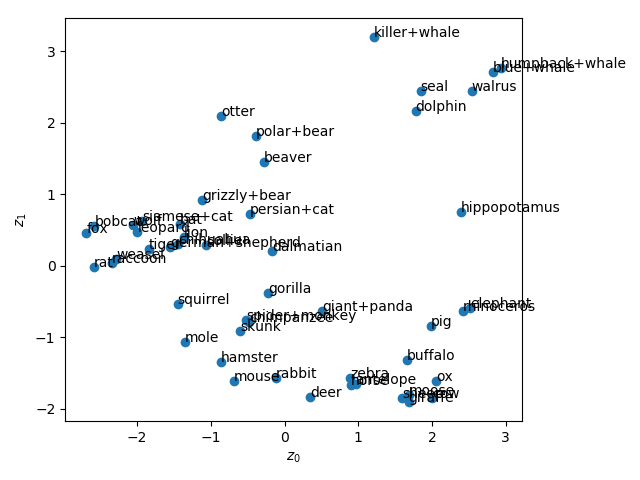
\includegraphics[scale = 0.5]{PCAvis11.png}\\

\subsection{Data Compression}

\enum{
\item $30.19\%$ of the variance is explained
\item We need at least $k \geq 5$. 
}


\subsection{Multi-Dimensional Scaling}

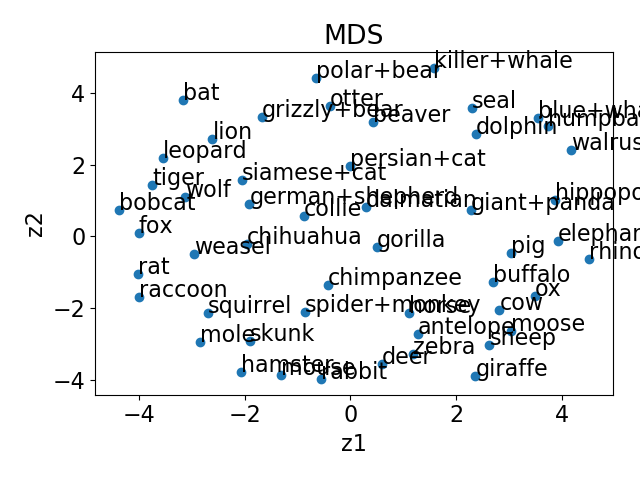
\includegraphics[scale=0.7]{../figs/MDS_animals.png}

\subsection{ISOMAP}

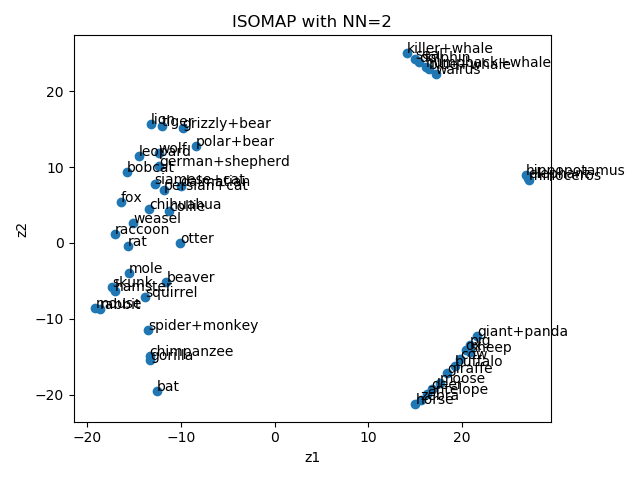
\includegraphics[scale=0.7]{ISOMAP2_animals.png}\\
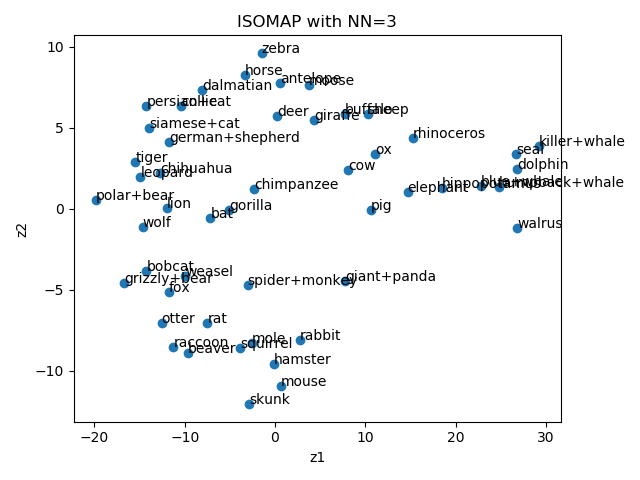
\includegraphics[scale=0.7]{ISOMAP3_animals.png}\\

\subsection{t-SNE}

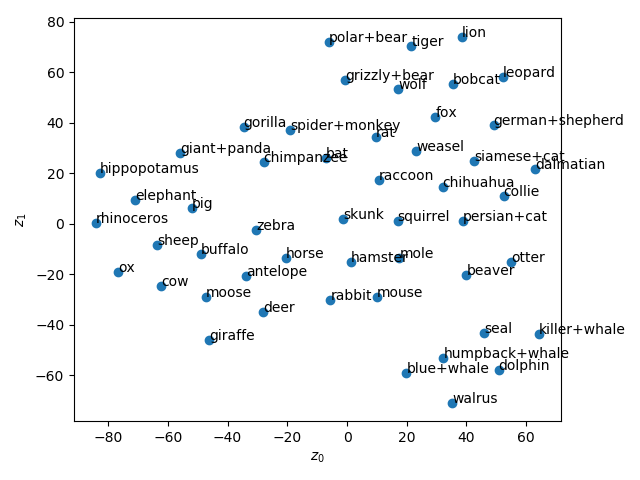
\includegraphics[scale=0.5]{TSNE.png}\\
All the plots have relatively scattered points on the graph so it is difficult to differentiate them. The best method would
be ISOMAP with $k=2$ because it does a relatively good job of grouping together the animals.

\subsection{Sensitivity to Initialization}

MDS is sensitive to initializations and so is t-SNE because t-SNE is a special case of MDS. In the graphs, we see
that this is true for t-SNE, which matches up with what we said in lectures. Our MDS is not sensitive to initializations
because our implementation initializes MDS the same way every time. 

\section{Neural Networks}

\subsection{Neural Networks by Hand}

$$
z_i = \mat{0 \\1}, h(z_i) = \mat{\frac12 \\\frac{1}{1+e^{-1}}}, y_i= \mat{\frac32 + \frac{1}{1+e^{-1}}}.
$$

\subsection{SGD for a Neural Network: implementation}

Training error =  0.08624
Test error     =  0.0839

\subsection{SGD for a Neural Network: discussion}

I think that the SGD implementation is definetely better as its run time is a tenth of the run time of GD implementation.
Although GD is about 3\% better in terms of accuracy, it is just too slow for large datasets like this one.

\subsection{Hyperparameter Tuning}

hidden layers = 100, alpha = 0.001\\
Training error =  0.00546
Test error     =  0.0276\\

hidden layers = 100, alpha = 0.01\\
Training error =  0.00144
Test error     =  0.0216\\

hidden layers = 100, alpha = 0.1\\
Training error =  0.00684
Test error     =  0.0212\\

hidden layers = 1, alpha = 0.0001\\
Training error =  0.59898
Test error     =  0.605\\

hidden layers = 200, alpha = 0.0001\\
Training error =  0.0074
Test error     =  0.0211\\

hidden layers = 300, alpha = 0.0001\\
Training error =  0.00656
Test error     =  0.0198\\

hidden layers = 400, alpha = 0.0001\\
Training error =  0.00636
Test error     =  0.0204\\

\section{Very-Short Answer Questions}

\begin{enumerate}
\item Yes
\item We can enforce regions that are convex and we may want elements of w to be non-negative.
\item ISOMAP is mainly used for unsupervised learning and it is non-parametric as it first finds the nearest neighbours
similar to that of KNN. 
\item Content-based filtering is better for new users because it can extract features of users to build a model and 
use that to predict for new users. Collaborative filtering is bad for new users because they have not rated anything 
so it will be hard to predict. 
\item Collaborative filtering uses L2 regularization and uses stochastic gradient descent. 
\item Neural Networks are used for supervised learning to learn features $z_i$ and it is parametric.
\item Regularization helps with reducing overfitting as we add more layers.
\item IDK
\item $10 \times 100 + 100 \times 3 + 100 + 3 = 1403$
\item The neural network will be convex as long as there are no hidden layers. For example, hidden\_layer\_sizes $= 0$, activation $=$ relu,
solver $=$ adam, alpha $= 0.0001$, batch\_size $= 200$, learning\_rate $=$ constant, number\_of\_epochs $= 10$, weight\_initialization $=$ random 
\item The vanishing gradient problem is that the parameters may underflow or overflow during the calculation of the gradient.
\item Convolutional neural networks has weight matrices that have a particular pattern of sparsity which reduces the number
of parameters. 
\end{enumerate}


\end{document}
